\subsection{Discovering Reciprocal Mixing: A Fun Exploration!}

\begin{tcolorbox}[colback=gray!10, colframe=black, title=E4C13]
What is reciprocal mixing? 

\begin{enumerate}[label=\Alph*.]
    \item Two out-of-band signals mixing to generate an in-band spurious signal
    \item In-phase signals cancelling in a mixer resulting in loss of receiver sensitivity
    \item Two digital signals combining from alternate time slots
    \item \textbf{Local oscillator phase noise mixing with adjacent strong signals to create interference to desired signals}
\end{enumerate} \end{tcolorbox}

\subsubsection{Understanding Reciprocal Mixing}

Reciprocal mixing is a phenomenon that occurs in radio frequency (RF) systems, particularly in the context of radio receivers. It involves the interaction between phase noise generated by a local oscillator and strong adjacent signals in the spectrum. 

When the local oscillator (LO) phase noise combines with these adjacent strong signals, it can create unwanted interference within the bandwidth of the desired signal, thus degrading receiver performance.

\subsubsection{Concepts Related to Reciprocal Mixing}

To understand reciprocal mixing fully, a reader should be familiar with several foundational concepts in radio communication:

1. \textbf{Local Oscillator (LO)}: In a superheterodyne receiver, the LO is an oscillator that shifts the frequency of incoming signals so they can be mixed down to a lower intermediate frequency (IF) for processing. The phase noise in the LO can contribute to interference in the presence of strong signals.

2. \textbf{Phase Noise}: This refers to the rapid, short-term variations in the phase of a signal. In an LO, phase noise can be problematic as it spreads out the power of the signal, possibly overlapping with adjacent channels.

3. \textbf{Mixer}: A circuit that combines two signals, producing new frequencies that are the sum and difference of the original frequencies. In this context, we are particularly concerned with how the LO's phase noise interacts in the mixer.

4. \textbf{Adjacent Strong Signals}: These are signals close in frequency to the desired signal, which can dominate the mixing process and cause interference when the LO phase noise is significant.

\subsubsection{Deriving the Effect of Reciprocal Mixing}

To illustrate reciprocal mixing mathematically, let's consider a simple model. Let \(f_{LO}\) be the local oscillator frequency and \(f_{adj}\) the frequency of an adjacent strong signal. The output from a mixer can be expressed as:

\[
P_{out} = P_{signal} \cdot P_{noise}
\]

Where \(P_{out}\) is the power of the unwanted signal generated due to mixing, \(P_{signal}\) is the power of the adjacent strong signal, and \(P_{noise}\) is derived from the phase noise of the LO. 

As the power of the adjacent signal increases, the generated interference can potentially rise to levels that disrupt the desired signal:

\[
P_{interference} = k \cdot P_{adj} \cdot \Delta f
\]

Where \(k\) is a constant that depends on the mixer design and \(\Delta f\) indicates the bandwidth affected by the phase noise.

In a practical scenario, an engineer will want to minimize \(P_{interference}\) by either improving the local oscillator's phase noise performance or implementing filtering techniques to suppress unwanted interference from strong adjacent signals.

\subsubsection{Diagrammatic Representation of Reciprocal Mixing}

\begin{center}
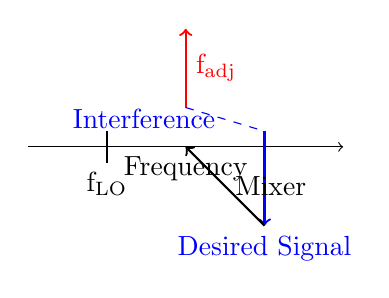
\begin{tikzpicture}
    \draw[->] (0,0) -- (4,0) node[midway, below] {Frequency};
    \draw (1,0.2) -- (1,-0.2) node[below] {f\textsubscript{LO}};
    \draw[red, thick, ->] (2,0.5) -- (2,1.5) node[midway, right] {f\textsubscript{adj}};
    \draw[blue, thick, ->] (3,0.2) -- (3,-1) node[below] {Desired Signal};
    \draw[blue, dashed] (2,0.5) -- (3,0.2) node[midway, left] {Interference};
    \draw[->, thick] (3,-1) -- (2,0) node[midway, above, right] {Mixer};
\end{tikzpicture}
\end{center}
